\documentclass[]{book}
\usepackage{lmodern}
\usepackage{amssymb,amsmath}
\usepackage{ifxetex,ifluatex}
\usepackage{fixltx2e} % provides \textsubscript
\ifnum 0\ifxetex 1\fi\ifluatex 1\fi=0 % if pdftex
  \usepackage[T1]{fontenc}
  \usepackage[utf8]{inputenc}
\else % if luatex or xelatex
  \ifxetex
    \usepackage{mathspec}
  \else
    \usepackage{fontspec}
  \fi
  \defaultfontfeatures{Ligatures=TeX,Scale=MatchLowercase}
\fi
% use upquote if available, for straight quotes in verbatim environments
\IfFileExists{upquote.sty}{\usepackage{upquote}}{}
% use microtype if available
\IfFileExists{microtype.sty}{%
\usepackage{microtype}
\UseMicrotypeSet[protrusion]{basicmath} % disable protrusion for tt fonts
}{}
\usepackage[margin=1in]{geometry}
\usepackage{hyperref}
\hypersetup{unicode=true,
            pdftitle={Finn 6211 - Final Project},
            pdfauthor={Davis Vaughan},
            pdfborder={0 0 0},
            breaklinks=true}
\urlstyle{same}  % don't use monospace font for urls
\usepackage{natbib}
\bibliographystyle{apalike}
\usepackage{color}
\usepackage{fancyvrb}
\newcommand{\VerbBar}{|}
\newcommand{\VERB}{\Verb[commandchars=\\\{\}]}
\DefineVerbatimEnvironment{Highlighting}{Verbatim}{commandchars=\\\{\}}
% Add ',fontsize=\small' for more characters per line
\usepackage{framed}
\definecolor{shadecolor}{RGB}{248,248,248}
\newenvironment{Shaded}{\begin{snugshade}}{\end{snugshade}}
\newcommand{\AlertTok}[1]{\textcolor[rgb]{0.94,0.16,0.16}{#1}}
\newcommand{\AnnotationTok}[1]{\textcolor[rgb]{0.56,0.35,0.01}{\textbf{\textit{#1}}}}
\newcommand{\AttributeTok}[1]{\textcolor[rgb]{0.77,0.63,0.00}{#1}}
\newcommand{\BaseNTok}[1]{\textcolor[rgb]{0.00,0.00,0.81}{#1}}
\newcommand{\BuiltInTok}[1]{#1}
\newcommand{\CharTok}[1]{\textcolor[rgb]{0.31,0.60,0.02}{#1}}
\newcommand{\CommentTok}[1]{\textcolor[rgb]{0.56,0.35,0.01}{\textit{#1}}}
\newcommand{\CommentVarTok}[1]{\textcolor[rgb]{0.56,0.35,0.01}{\textbf{\textit{#1}}}}
\newcommand{\ConstantTok}[1]{\textcolor[rgb]{0.00,0.00,0.00}{#1}}
\newcommand{\ControlFlowTok}[1]{\textcolor[rgb]{0.13,0.29,0.53}{\textbf{#1}}}
\newcommand{\DataTypeTok}[1]{\textcolor[rgb]{0.13,0.29,0.53}{#1}}
\newcommand{\DecValTok}[1]{\textcolor[rgb]{0.00,0.00,0.81}{#1}}
\newcommand{\DocumentationTok}[1]{\textcolor[rgb]{0.56,0.35,0.01}{\textbf{\textit{#1}}}}
\newcommand{\ErrorTok}[1]{\textcolor[rgb]{0.64,0.00,0.00}{\textbf{#1}}}
\newcommand{\ExtensionTok}[1]{#1}
\newcommand{\FloatTok}[1]{\textcolor[rgb]{0.00,0.00,0.81}{#1}}
\newcommand{\FunctionTok}[1]{\textcolor[rgb]{0.00,0.00,0.00}{#1}}
\newcommand{\ImportTok}[1]{#1}
\newcommand{\InformationTok}[1]{\textcolor[rgb]{0.56,0.35,0.01}{\textbf{\textit{#1}}}}
\newcommand{\KeywordTok}[1]{\textcolor[rgb]{0.13,0.29,0.53}{\textbf{#1}}}
\newcommand{\NormalTok}[1]{#1}
\newcommand{\OperatorTok}[1]{\textcolor[rgb]{0.81,0.36,0.00}{\textbf{#1}}}
\newcommand{\OtherTok}[1]{\textcolor[rgb]{0.56,0.35,0.01}{#1}}
\newcommand{\PreprocessorTok}[1]{\textcolor[rgb]{0.56,0.35,0.01}{\textit{#1}}}
\newcommand{\RegionMarkerTok}[1]{#1}
\newcommand{\SpecialCharTok}[1]{\textcolor[rgb]{0.00,0.00,0.00}{#1}}
\newcommand{\SpecialStringTok}[1]{\textcolor[rgb]{0.31,0.60,0.02}{#1}}
\newcommand{\StringTok}[1]{\textcolor[rgb]{0.31,0.60,0.02}{#1}}
\newcommand{\VariableTok}[1]{\textcolor[rgb]{0.00,0.00,0.00}{#1}}
\newcommand{\VerbatimStringTok}[1]{\textcolor[rgb]{0.31,0.60,0.02}{#1}}
\newcommand{\WarningTok}[1]{\textcolor[rgb]{0.56,0.35,0.01}{\textbf{\textit{#1}}}}
\usepackage{longtable,booktabs}
\usepackage{graphicx,grffile}
\makeatletter
\def\maxwidth{\ifdim\Gin@nat@width>\linewidth\linewidth\else\Gin@nat@width\fi}
\def\maxheight{\ifdim\Gin@nat@height>\textheight\textheight\else\Gin@nat@height\fi}
\makeatother
% Scale images if necessary, so that they will not overflow the page
% margins by default, and it is still possible to overwrite the defaults
% using explicit options in \includegraphics[width, height, ...]{}
\setkeys{Gin}{width=\maxwidth,height=\maxheight,keepaspectratio}
\IfFileExists{parskip.sty}{%
\usepackage{parskip}
}{% else
\setlength{\parindent}{0pt}
\setlength{\parskip}{6pt plus 2pt minus 1pt}
}
\setlength{\emergencystretch}{3em}  % prevent overfull lines
\providecommand{\tightlist}{%
  \setlength{\itemsep}{0pt}\setlength{\parskip}{0pt}}
\setcounter{secnumdepth}{5}
% Redefines (sub)paragraphs to behave more like sections
\ifx\paragraph\undefined\else
\let\oldparagraph\paragraph
\renewcommand{\paragraph}[1]{\oldparagraph{#1}\mbox{}}
\fi
\ifx\subparagraph\undefined\else
\let\oldsubparagraph\subparagraph
\renewcommand{\subparagraph}[1]{\oldsubparagraph{#1}\mbox{}}
\fi

%%% Use protect on footnotes to avoid problems with footnotes in titles
\let\rmarkdownfootnote\footnote%
\def\footnote{\protect\rmarkdownfootnote}

%%% Change title format to be more compact
\usepackage{titling}

% Create subtitle command for use in maketitle
\newcommand{\subtitle}[1]{
  \posttitle{
    \begin{center}\large#1\end{center}
    }
}

\setlength{\droptitle}{-2em}
  \title{Finn 6211 - Final Project}
  \pretitle{\vspace{\droptitle}\centering\huge}
  \posttitle{\par}
  \author{Davis Vaughan}
  \preauthor{\centering\large\emph}
  \postauthor{\par}
  \predate{\centering\large\emph}
  \postdate{\par}
  \date{2018-04-17}

\usepackage{booktabs}

\usepackage{amsthm}
\newtheorem{theorem}{Theorem}[chapter]
\newtheorem{lemma}{Lemma}[chapter]
\theoremstyle{definition}
\newtheorem{definition}{Definition}[chapter]
\newtheorem{corollary}{Corollary}[chapter]
\newtheorem{proposition}{Proposition}[chapter]
\theoremstyle{definition}
\newtheorem{example}{Example}[chapter]
\theoremstyle{definition}
\newtheorem{exercise}{Exercise}[chapter]
\theoremstyle{remark}
\newtheorem*{remark}{Remark}
\newtheorem*{solution}{Solution}
\begin{document}
\maketitle

{
\setcounter{tocdepth}{1}
\tableofcontents
}
\hypertarget{titlepage}{%
\chapter{Introduction}\label{titlepage}}

This is the final project of the Finn 6211 class, with the intention of
getting comfortable with spot rate data, their relation to yield curve
factors, and various hedging strategies.

The instructions for the report can be found
\href{./instructions/Hedging_Project_S18.pdf}{here}.

An R package has been created to accompany the report. It contains a
number of helper functions for cleaning data, manipulating the time
series, and creating the hedging strategies. The package is named
\texttt{ratekit} and can be found on Github
\href{https://github.com/DavisVaughan/ratekit}{here}.

The book is intended to provide a summary of the methods used in the
project. In each section of the book is a link to the script that was
actually run to generate the results for the project. Those scripts are
more in depth and cover every aspect of the project.

This report was written with
\href{https://bookdown.org/yihui/bookdown/}{bookdown}, a book authoring
package for R.

\hypertarget{data}{%
\chapter{Data}\label{data}}

\hypertarget{retrieve}{%
\section{Getting the data}\label{retrieve}}

Script) \href{./R/01-download.R}{01-download.R}

The data is retrieved from the Federal Reserve website, under the
discussion series: \emph{The U.S. Treasury Yield Curve: 1961 to the
Present}. The link for that site is
\href{https://www.federalreserve.gov/pubs/feds/2006/200628/200628abs.html}{here}.
The specific data set that was downloaded was the XLS file included on
that site.

The data was immediately opened in Excel, and was resaved as an
\texttt{xlsx} file. The format of the data is not a true \texttt{xls}
file, instead it is some kind of \texttt{xml} file. This does not play
nicely with R's packages for importing Excel data, so a resave was
necessary and is done manually.

\texttt{ratekit} provides the \texttt{download\_rates\_xls()} helper
function for this.

\hypertarget{cleaning}{%
\section{Cleaning}\label{cleaning}}

Script) \href{./R/02-cleaning.R}{02-cleaning.R}

Data is brought in using the \texttt{readxl} package and the
\texttt{ratekit} helper, \texttt{read\_rates()}. This function reads the
rectangle of rates data only, and sets any \texttt{-999.99} values to
\texttt{NA}. These are often found through the dataset, and I assume
they are meant to represent missing values. To visualize the \texttt{NA}
values in the dataset, I use the \texttt{visdat} package.

First, let's look at what is immediately brought in by
\texttt{read\_rates()}. We will need a few packages throughout the
chapter, so let's load those now as well.

\begin{Shaded}
\begin{Highlighting}[]
\KeywordTok{library}\NormalTok{(visdat)}
\KeywordTok{library}\NormalTok{(ratekit)}
\KeywordTok{library}\NormalTok{(dplyr)}
\KeywordTok{library}\NormalTok{(tibbletime)}

\NormalTok{raw <-}\StringTok{ }\KeywordTok{read_rates}\NormalTok{(}\StringTok{"data/raw/feds200628.xlsx"}\NormalTok{)}

\NormalTok{raw}
\end{Highlighting}
\end{Shaded}

\begin{verbatim}
## # A tibble: 14,163 x 100
##   date       SVENY01 SVENY02 SVENY03 SVENY04 SVENY05 SVENY06 SVENY07
##   <date>       <dbl>   <dbl>   <dbl>   <dbl>   <dbl>   <dbl>   <dbl>
## 1 2018-03-29    2.10    2.27    2.40    2.49    2.56    2.62    2.66
## 2 2018-03-28    2.10    2.28    2.41    2.51    2.59    2.65    2.69
## 3 2018-03-27    2.09    2.26    2.40    2.50    2.58    2.64    2.69
## 4 2018-03-26    2.10    2.30    2.45    2.57    2.65    2.71    2.76
## 5 2018-03-23    2.09    2.27    2.42    2.53    2.61    2.68    2.73
## # ... with 1.416e+04 more rows, and 92 more variables: SVENY08 <dbl>,
## #   SVENY09 <dbl>, SVENY10 <dbl>, SVENY11 <dbl>, SVENY12 <dbl>,
## #   SVENY13 <dbl>, SVENY14 <dbl>, SVENY15 <dbl>, SVENY16 <dbl>,
## #   SVENY17 <dbl>, SVENY18 <dbl>, SVENY19 <dbl>, SVENY20 <dbl>,
## #   SVENY21 <dbl>, SVENY22 <dbl>, SVENY23 <dbl>, SVENY24 <dbl>,
## #   SVENY25 <dbl>, SVENY26 <dbl>, SVENY27 <dbl>, SVENY28 <dbl>,
## #   SVENY29 <dbl>, SVENY30 <dbl>, SVENPY01 <dbl>, SVENPY02 <dbl>,
## #   SVENPY03 <dbl>, SVENPY04 <dbl>, SVENPY05 <dbl>, SVENPY06 <dbl>,
## #   SVENPY07 <dbl>, SVENPY08 <dbl>, SVENPY09 <dbl>, SVENPY10 <dbl>,
## #   SVENPY11 <dbl>, SVENPY12 <dbl>, SVENPY13 <dbl>, SVENPY14 <dbl>,
## #   SVENPY15 <dbl>, SVENPY16 <dbl>, SVENPY17 <dbl>, SVENPY18 <dbl>,
## #   SVENPY19 <dbl>, SVENPY20 <dbl>, SVENPY21 <dbl>, SVENPY22 <dbl>,
## #   SVENPY23 <dbl>, SVENPY24 <dbl>, SVENPY25 <dbl>, SVENPY26 <dbl>,
## #   SVENPY27 <dbl>, SVENPY28 <dbl>, SVENPY29 <dbl>, SVENPY30 <dbl>,
## #   SVENF01 <dbl>, SVENF02 <dbl>, SVENF03 <dbl>, SVENF04 <dbl>,
## #   SVENF05 <dbl>, SVENF06 <dbl>, SVENF07 <dbl>, SVENF08 <dbl>,
## #   SVENF09 <dbl>, SVENF10 <dbl>, SVENF11 <dbl>, SVENF12 <dbl>,
## #   SVENF13 <dbl>, SVENF14 <dbl>, SVENF15 <dbl>, SVENF16 <dbl>,
## #   SVENF17 <dbl>, SVENF18 <dbl>, SVENF19 <dbl>, SVENF20 <dbl>,
## #   SVENF21 <dbl>, SVENF22 <dbl>, SVENF23 <dbl>, SVENF24 <dbl>,
## #   SVENF25 <dbl>, SVENF26 <dbl>, SVENF27 <dbl>, SVENF28 <dbl>,
## #   SVENF29 <dbl>, SVENF30 <dbl>, SVEN1F01 <dbl>, SVEN1F04 <dbl>,
## #   SVEN1F09 <dbl>, BETA0 <dbl>, BETA1 <dbl>, BETA2 <dbl>, BETA3 <dbl>,
## #   TAU1 <dbl>, TAU2 <dbl>
\end{verbatim}

Not a bad start, but I'm worried about missing values. Also, what are
those column names?

The column names in the data correspond to different types and lengths
of rates used in the paper. The key for understanding the column names
is below:

\begin{tabular}{l|l|l}
\hline
series & compounding\_convention & key\\
\hline
Zero-coupon yield & Continuously Compounded & SVENYXX\\
\hline
Par yield & Coupon-Equivalent & SVENPYXX\\
\hline
Instantaneous forward rate & Continuously Compounded & SVENFXX\\
\hline
One-year forward rate & Coupon-Equivalent & SVEN1FXX\\
\hline
Parameters & NA & BETA0 to TAU2\\
\hline
\end{tabular}

Using \texttt{vis\_dat()}, we can take a look at our dataset all at once
to determine which data points to exclude.

\begin{Shaded}
\begin{Highlighting}[]
\KeywordTok{vis_dat}\NormalTok{(raw, }\DataTypeTok{warn_large_data =} \OtherTok{FALSE}\NormalTok{)}
\end{Highlighting}
\end{Shaded}

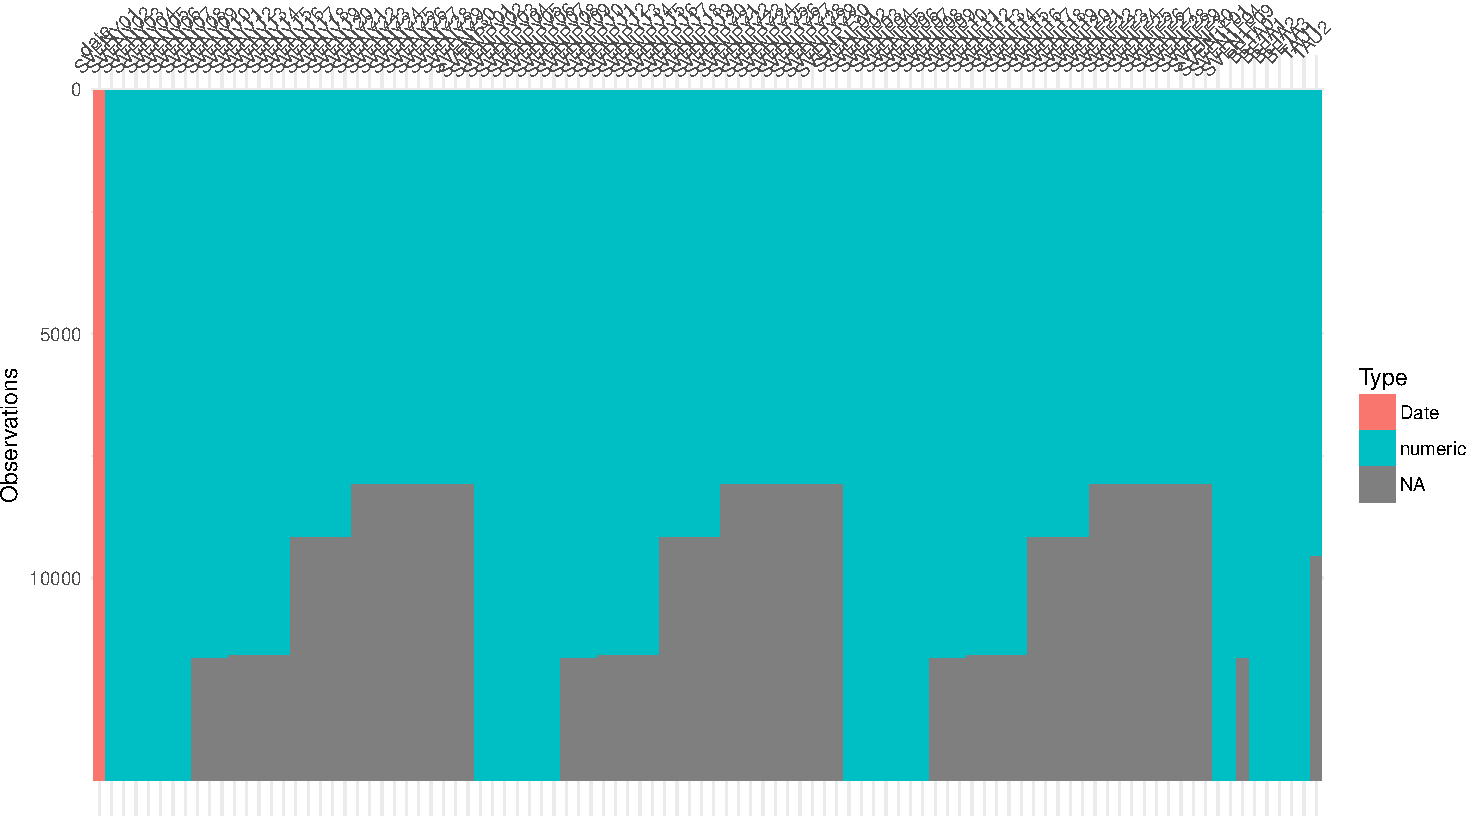
\includegraphics{final-project-book_files/figure-latex/missing_vals-1.pdf}

A clear pattern is seen in the missing values, with the number of
missing values increasing as you go further back in time and look at
longer rates (10 year VS 30 year). This might be a bit difficult to see
if you look at everything, but becomes clearer if you zoom in on just
one set of series.

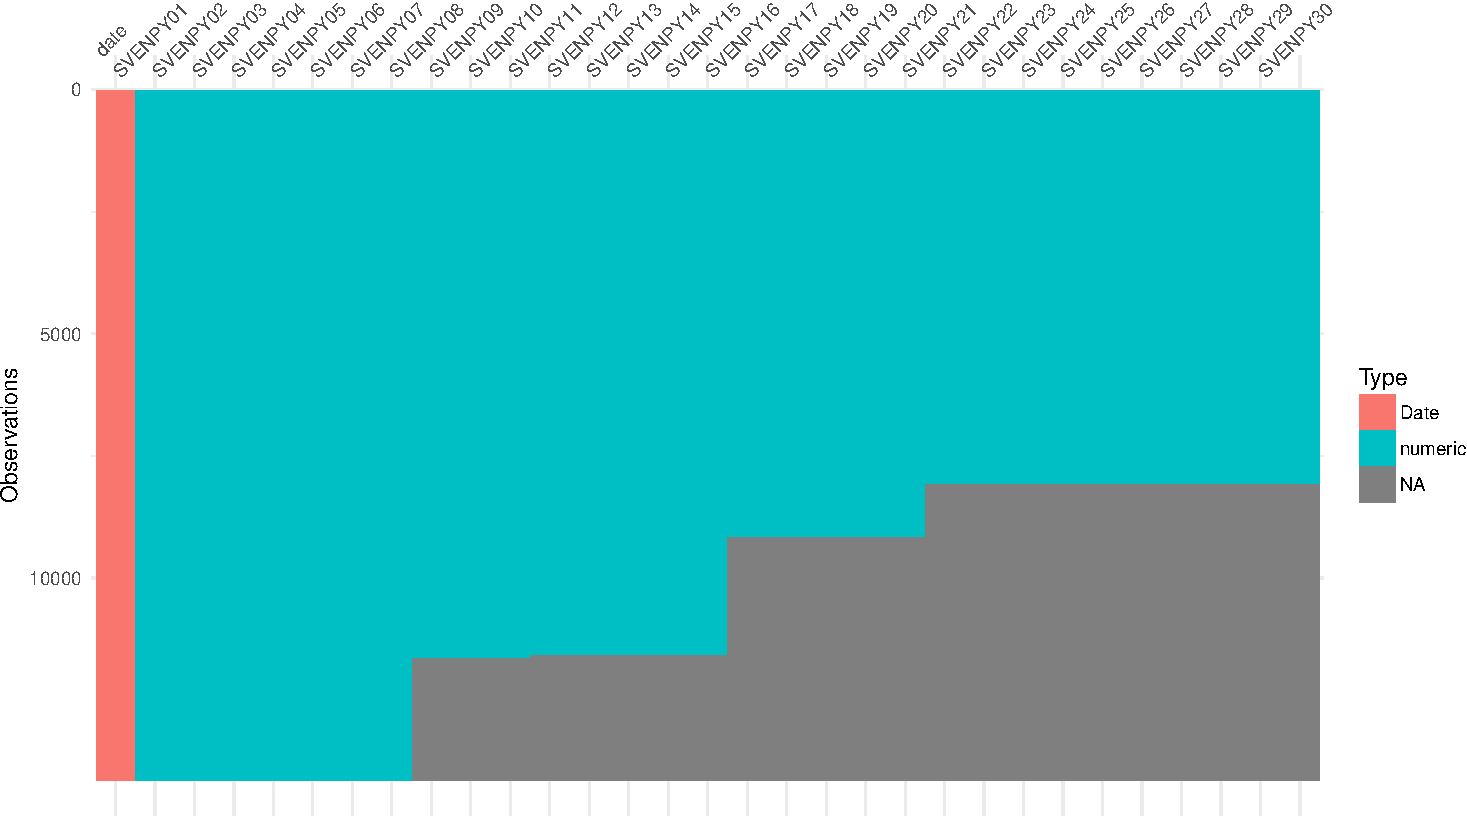
\includegraphics{final-project-book_files/figure-latex/par_yield_missing-1.pdf}

The parameters are affected by this as well, but not as much, with only
\texttt{TAU2} being affected.

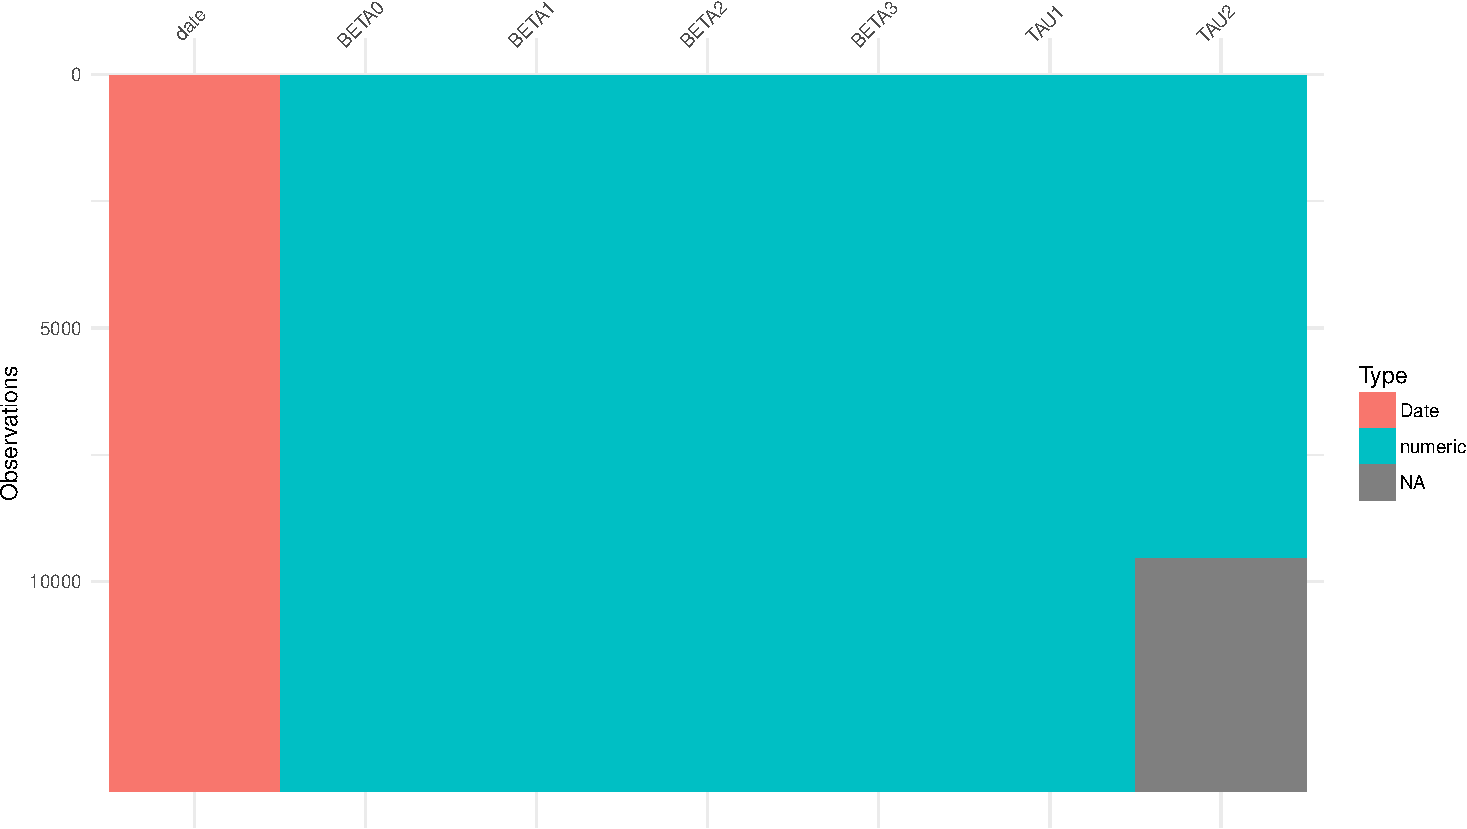
\includegraphics{final-project-book_files/figure-latex/parameters_missing-1.pdf}

Since the parameters are all we care about for this project, I decided
to throw out any row with an \texttt{NA} value for \texttt{TAU2}. This
threw out every data point before 1980. We can ensure that we don't have
any missing values now with \texttt{vis\_miss()}.

\begin{Shaded}
\begin{Highlighting}[]
\CommentTok{# This is the cleaned parameter set, cleaned using 02-cleaning.R}
\NormalTok{parameters <-}\StringTok{ }\KeywordTok{readRDS}\NormalTok{(}\StringTok{"data/cleaned/parameters/parameters.rds"}\NormalTok{)}
\KeywordTok{vis_miss}\NormalTok{(parameters)}
\end{Highlighting}
\end{Shaded}

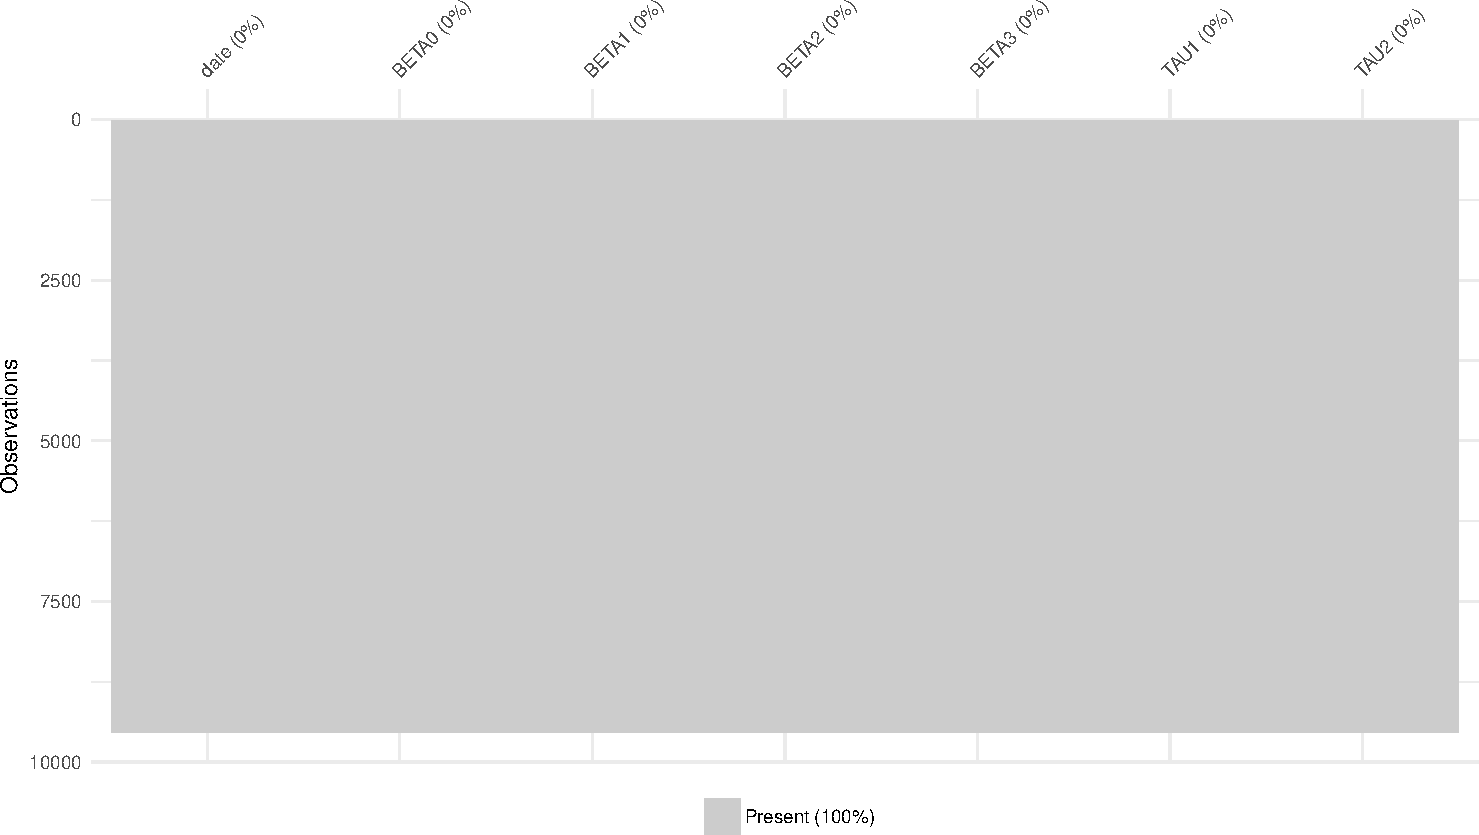
\includegraphics{final-project-book_files/figure-latex/parameters_clean-1.pdf}

\hypertarget{monthly}{%
\section{Monthly and Ascending}\label{monthly}}

Script)
\href{./R/03-to-monthly-and-ascending.R}{03-to-monthly-and-ascending.R}

At this point, our dataset looks like this:

\begin{Shaded}
\begin{Highlighting}[]
\NormalTok{parameters <-}\StringTok{ }\KeywordTok{readRDS}\NormalTok{(}\StringTok{"data/cleaned/parameters/parameters.rds"}\NormalTok{)}
\NormalTok{parameters}
\end{Highlighting}
\end{Shaded}

\begin{verbatim}
## # A tibble: 9,543 x 7
##   date       BETA0 BETA1      BETA2 BETA3  TAU1  TAU2
##   <date>     <dbl> <dbl>      <dbl> <dbl> <dbl> <dbl>
## 1 2018-03-29  4.13 -2.25  0.000228  -3.07  2.84  11.4
## 2 2018-03-28  4.35 -2.48 -0.000089  -3.53  2.99  12.2
## 3 2018-03-27  4.44 -2.59  0.000314  -3.67  3.18  12.5
## 4 2018-03-26  4.27 -2.44 -0.0000588 -3.12  2.73  11.8
## 5 2018-03-23  4.53 -2.69  0.000245  -3.78  3.17  12.9
## # ... with 9,538 more rows
\end{verbatim}

We want monthly data, and we will need to put it in ascending order. We
can convert to monthly with \texttt{as\_period()} from
\texttt{tibbletime}, and arrange it by ascending date with
\texttt{arrange()} from \texttt{dplyr}.

\begin{Shaded}
\begin{Highlighting}[]
\NormalTok{parameters_monthly <-}\StringTok{ }\NormalTok{parameters }\OperatorTok
\StringTok{  }\KeywordTok{as_tbl_time}\NormalTok{(date) }\OperatorTok
\StringTok{  }\KeywordTok{arrange}\NormalTok{(date) }\OperatorTok\StringTok{ }
\StringTok{  }\KeywordTok{as_period}\NormalTok{(}\StringTok{"monthly"}\NormalTok{, }\DataTypeTok{side =} \StringTok{"end"}\NormalTok{)}

\NormalTok{parameters_monthly}
\end{Highlighting}
\end{Shaded}

\begin{verbatim}
## # A time tibble: 459 x 7
## # Index: date
##   date       BETA0  BETA1 BETA2 BETA3  TAU1  TAU2
##   <date>     <dbl>  <dbl> <dbl> <dbl> <dbl> <dbl>
## 1 1980-01-31  11.8  0.979 -622.  617.  2.50  2.50
## 2 1980-02-29  11.8  1.53  -617.  621.  1.15  1.15
## 3 1980-03-31  13.2  2.95  -622.  617.  1.78  1.76
## 4 1980-04-30  11.1  0.607 -621.  617.  1.59  1.59
## 5 1980-05-30  11.3 -3.44  -620.  618.  1.36  1.35
## # ... with 454 more rows
\end{verbatim}

This leaves us with 459 rows of data for our project, spanning
1980-01-31 to 2018-03-29.

\hypertarget{rates}{%
\chapter{Fixed Income Features Calculations}\label{rates}}

In this chapter, I will construct spot rates, zero coupon bond prices,
excess returns, and yield factors. These features will be used later in
hedging strategies and for general exploration of the data.

The following packages are required in this chapter.

\begin{Shaded}
\begin{Highlighting}[]
\KeywordTok{library}\NormalTok{(readr)}
\KeywordTok{library}\NormalTok{(ratekit)}
\KeywordTok{library}\NormalTok{(dplyr)}
\end{Highlighting}
\end{Shaded}

\hypertarget{spot-rates}{%
\section{Spot Rates}\label{spot-rates}}

Script)
\href{./R/04-spot-rates-and-prices.R}{04-spot-rates-and-prices.R}

Spot rates series can be constructed from the 6 parameters in the rates
dataset. The following formula is used to construct the spot rates. It
is integrated form of the Svensson extension of the Nelson and Siegal
approach to calculating instantaneous forward rates. Svensson added a
second hump term to the model that Nelson and Siegal created.
Integrating the instantaneous forward rates gives us the spot rates.

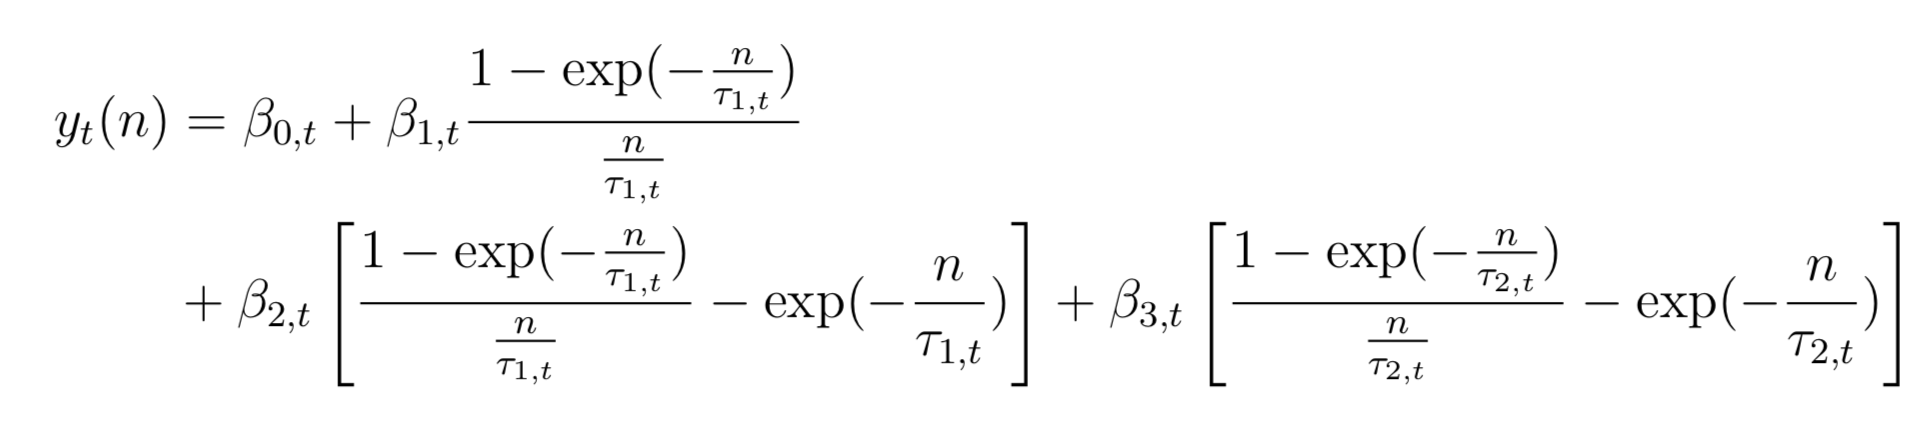
\includegraphics[width=26.67in]{images/spot-rates}

To reconstruct this, I used a programming concept known as a
\emph{function factory}. This is a specialized function that returns a
function. This extends naturally to this use case because the outer
function can accept the time series of the 6 parameters, and the inner
function that get's returned is parameterized by \texttt{n},
corresponding to the n-year spot rate at time t. The
\texttt{spot\_rate\_factory()} function lives in \texttt{ratekit}, and
looks like this.

\begin{Shaded}
\begin{Highlighting}[]
\NormalTok{spot_rate_factory}
\end{Highlighting}
\end{Shaded}

\begin{verbatim}
## function(beta_0, beta_1, beta_2, beta_3, tau_1, tau_2) {
## 
##   # Spot rate function based on Equation 22 of
##   # Gurkaynak, Sack and Wright (2006)
##   spot_rate_n <- function(n) {
## 
##     spot_rate_percentage <-
##     beta_0 +
##     beta_1 *  (1 - exp( -n / tau_1)) / (n / tau_1) +
##     beta_2 * ((1 - exp( -n / tau_1)) / (n / tau_1) - exp( -n / tau_1)) +
##     beta_3 * ((1 - exp( -n / tau_2)) / (n / tau_2) - exp( -n / tau_2))
## 
##     spot_rate_percentage / 100
##   }
## 
## 
##   spot_rate_n
## }
## <environment: namespace:ratekit>
\end{verbatim}

As you can see, it accepts the 6 parameters, and returns a function
parameterized by \texttt{n}. Because we want to calculate the spot rate
for a number of different years, this parameterized function will be
very useful. Below is an example usage of this concept.

\begin{Shaded}
\begin{Highlighting}[]
\CommentTok{# The monthly parameters from the Data chapter}
\NormalTok{parameters_monthly <-}\StringTok{ }\KeywordTok{read_rds}\NormalTok{(}\StringTok{"data/cleaned/parameters/parameters_monthly.rds"}\NormalTok{)}

\CommentTok{# The generated function. The function signature is generate_spot_rates(n)}
\NormalTok{generate_spot_rates <-}\StringTok{ }\KeywordTok{with}\NormalTok{(}
  \DataTypeTok{data =}\NormalTok{ parameters_monthly, }
  \DataTypeTok{expr =} \KeywordTok{spot_rate_factory}\NormalTok{(BETA0, BETA1, BETA2, BETA3, TAU1, TAU2)}
\NormalTok{)}

\CommentTok{# Calculate the series of 1/12 year, 11/12 year, and 1 year spot rates}
\NormalTok{spot_rates <-}\StringTok{ }\NormalTok{parameters_monthly }\OperatorTok
\StringTok{  }\KeywordTok{select}\NormalTok{(date) }\OperatorTok
\StringTok{  }\KeywordTok{mutate}\NormalTok{(}
    \DataTypeTok{spot_1_month  =} \KeywordTok{generate_spot_rates}\NormalTok{(}\DecValTok{1}\OperatorTok{/}\DecValTok{12}\NormalTok{),}
    \DataTypeTok{spot_11_month =} \KeywordTok{generate_spot_rates}\NormalTok{(}\DecValTok{11}\OperatorTok{/}\DecValTok{12}\NormalTok{),}
    \DataTypeTok{spot_12_month =} \KeywordTok{generate_spot_rates}\NormalTok{(}\DecValTok{1}\NormalTok{)}
\NormalTok{  )}

\NormalTok{spot_rates}
\end{Highlighting}
\end{Shaded}

\begin{verbatim}
## # A time tibble: 459 x 4
## # Index: date
##   date       spot_1_month spot_11_month spot_12_month
##   <date>            <dbl>         <dbl>         <dbl>
## 1 1980-01-31       0.126         0.118         0.118 
## 2 1980-02-29       0.136         0.145         0.145 
## 3 1980-03-31       0.161         0.152         0.151 
## 4 1980-04-30       0.116         0.107         0.107 
## 5 1980-05-30       0.0795        0.0867        0.0871
## # ... with 454 more rows
\end{verbatim}

\hypertarget{zero-coupon-bond-prices}{%
\section{Zero Coupon Bond Prices}\label{zero-coupon-bond-prices}}

Script)
\href{./R/04-spot-rates-and-prices.R}{04-spot-rates-and-prices.R}

n-year zero coupon bond prices can be calculated easily from their
corresponding spot rates. Below is the relationship between the two.

\begin{center}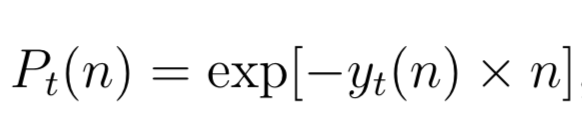
\includegraphics[width=8.08in]{images/zero-prices} \end{center}

Like for the spot rates, a function factory was constructed that
accepted the spot rate function, and returned a function that calculates
a vector of bond prices parameterized by \texttt{n}.

\begin{Shaded}
\begin{Highlighting}[]
\NormalTok{zero_bond_price_factory}
\end{Highlighting}
\end{Shaded}

\begin{verbatim}
## function(spot_rate_fn) {
## 
##   # Zero coupon bond for 1 dollar is just discounted spot rate
##   zero_bond_price_fn <- function(n) {
##     exp( - spot_rate_fn(n) * n)
##   }
## 
##   zero_bond_price_fn
## }
## <environment: namespace:ratekit>
\end{verbatim}

Using this relationship, the zero coupon bond prices were computed as
the following:

\begin{Shaded}
\begin{Highlighting}[]
\NormalTok{generate_zero_prices <-}\StringTok{ }\KeywordTok{zero_bond_price_factory}\NormalTok{(generate_spot_rates)}

\NormalTok{zero_prices <-}\StringTok{ }\NormalTok{spot_rates }\OperatorTok
\StringTok{  }\KeywordTok{transmute}\NormalTok{(}
\NormalTok{    date, }
    \DataTypeTok{zero_prices_1_month =} \KeywordTok{generate_zero_prices}\NormalTok{(}\DecValTok{1}\OperatorTok{/}\DecValTok{12}\NormalTok{),}
    \DataTypeTok{zero_prices_11_month =} \KeywordTok{generate_zero_prices}\NormalTok{(}\DecValTok{11}\OperatorTok{/}\DecValTok{12}\NormalTok{),}
    \DataTypeTok{zero_prices_12_month =} \KeywordTok{generate_zero_prices}\NormalTok{(}\DecValTok{1}\NormalTok{)}
\NormalTok{  )}

\NormalTok{zero_prices}
\end{Highlighting}
\end{Shaded}

\begin{verbatim}
## # A time tibble: 459 x 4
## # Index: date
##   date       zero_prices_1_month zero_prices_11_month zero_prices_12_month
##   <date>                   <dbl>                <dbl>                <dbl>
## 1 1980-01-31               0.990                0.897                0.889
## 2 1980-02-29               0.989                0.875                0.865
## 3 1980-03-31               0.987                0.870                0.860
## 4 1980-04-30               0.990                0.906                0.899
## 5 1980-05-30               0.993                0.924                0.917
## # ... with 454 more rows
\end{verbatim}

\hypertarget{one-month-returns}{%
\section{One Month Returns}\label{one-month-returns}}

Script) \href{./R/05-returns.R}{05-returns.R}

The time \(t+\Delta\) return on a n-year bond is:

\begin{center}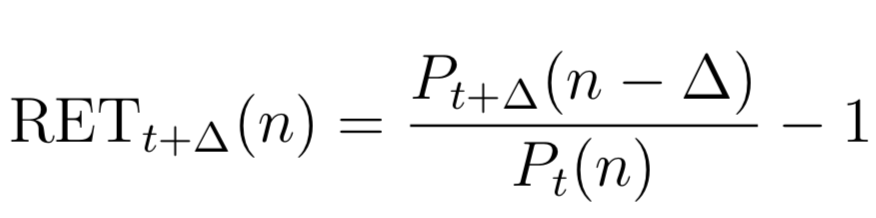
\includegraphics[width=12.17in]{images/returns} \end{center}

Using the zero bond prices from before, it is easy to calculate returns.
For example, 1 month returns for 1 year zero coupon bonds can be
calculated as:

\begin{Shaded}
\begin{Highlighting}[]
\NormalTok{returns <-}\StringTok{ }\NormalTok{zero_prices }\OperatorTok
\StringTok{  }\KeywordTok{mutate}\NormalTok{(}
    \DataTypeTok{zero_prices_12_month_lag =} \KeywordTok{lag}\NormalTok{(zero_prices_}\DecValTok{12}\NormalTok{_month),}
    \DataTypeTok{one_month_return =}\NormalTok{ zero_prices_}\DecValTok{11}\NormalTok{_month }\OperatorTok{/}\StringTok{ }\NormalTok{zero_prices_}\DecValTok{12}\NormalTok{_month_lag }\OperatorTok{-}\StringTok{ }\DecValTok{1}
\NormalTok{  ) }\OperatorTok\StringTok{ }
\StringTok{  }\KeywordTok{select}\NormalTok{(}\OperatorTok{-}\NormalTok{zero_prices_}\DecValTok{1}\NormalTok{_month, }\OperatorTok{-}\NormalTok{zero_prices_}\DecValTok{12}\NormalTok{_month_lag)}

\NormalTok{returns}
\end{Highlighting}
\end{Shaded}

\begin{verbatim}
## # A time tibble: 459 x 4
## # Index: date
##   date       zero_prices_11_month zero_prices_12_month one_month_return
##   <date>                    <dbl>                <dbl>            <dbl>
## 1 1980-01-31                0.897                0.889         NA      
## 2 1980-02-29                0.875                0.865         -0.0153 
## 3 1980-03-31                0.870                0.860          0.00574
## 4 1980-04-30                0.906                0.899          0.0543 
## 5 1980-05-30                0.924                0.917          0.0275 
## # ... with 454 more rows
\end{verbatim}

\hypertarget{excess-returns}{%
\section{Excess Returns}\label{excess-returns}}

Script) \href{./R/05-returns.R}{05-returns.R}

Excess returns are calculated over the 1 month treasury, specifically:

\begin{center}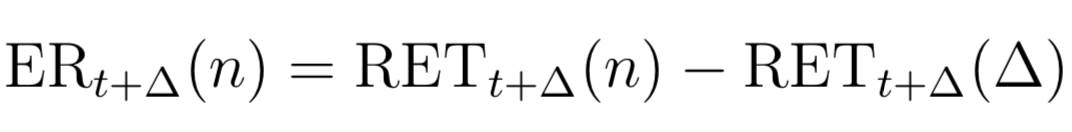
\includegraphics[width=14.89in]{images/excess-returns} \end{center}

For excess returns, the one month on the n-year bond must be calculated,
and the return on the benchmark (1 month treasury) must be calculated.
We already have 1-year bond returns, but we need to calculate our
benchmark returns. That can be done using the same formula as the 1-year
returns, but where \(P_{t+\Delta}(n-\Delta) = 1\), the maturity value.

\begin{Shaded}
\begin{Highlighting}[]
\NormalTok{returns_bench <-}\StringTok{ }\NormalTok{zero_prices }\OperatorTok
\StringTok{  }\KeywordTok{mutate}\NormalTok{(}\DataTypeTok{return_benchmark =} \DecValTok{1} \OperatorTok{/}\StringTok{ }\KeywordTok{lag}\NormalTok{(zero_prices_}\DecValTok{1}\NormalTok{_month) }\OperatorTok{-}\StringTok{ }\DecValTok{1}\NormalTok{) }\OperatorTok
\StringTok{  }\KeywordTok{select}\NormalTok{(date, zero_prices_}\DecValTok{1}\NormalTok{_month, return_benchmark)}

\NormalTok{returns_bench}
\end{Highlighting}
\end{Shaded}

\begin{verbatim}
## # A time tibble: 459 x 3
## # Index: date
##   date       zero_prices_1_month return_benchmark
##   <date>                   <dbl>            <dbl>
## 1 1980-01-31               0.990         NA      
## 2 1980-02-29               0.989          0.0106 
## 3 1980-03-31               0.987          0.0114 
## 4 1980-04-30               0.990          0.0135 
## 5 1980-05-30               0.993          0.00973
## # ... with 454 more rows
\end{verbatim}

With these two sets of returns in hand, we can calculate excess returns
for the one year bond.

\begin{Shaded}
\begin{Highlighting}[]
\NormalTok{excess_returns <-}\StringTok{ }\NormalTok{returns }\OperatorTok
\StringTok{  }\KeywordTok{left_join}\NormalTok{(returns_bench, }\StringTok{"date"}\NormalTok{) }\OperatorTok
\StringTok{  }\KeywordTok{transmute}\NormalTok{(date, }\DataTypeTok{excess_returns =}\NormalTok{ one_month_return }\OperatorTok{-}\StringTok{ }\NormalTok{return_benchmark)}

\NormalTok{excess_returns}
\end{Highlighting}
\end{Shaded}

\begin{verbatim}
## # A time tibble: 459 x 2
## # Index: date
##   date       excess_returns
##   <date>              <dbl>
## 1 1980-01-31       NA      
## 2 1980-02-29       -0.0259 
## 3 1980-03-31       -0.00568
## 4 1980-04-30        0.0408 
## 5 1980-05-30        0.0177 
## # ... with 454 more rows
\end{verbatim}

\hypertarget{yield-curve-factors}{%
\section{Yield Curve Factors}\label{yield-curve-factors}}

Script) \href{./R/06-yield-curve-factors.R}{06-yield-curve-factors.R}

Finally, the yield curve factors, level, slope, and curvature are
calculated as:

\begin{center}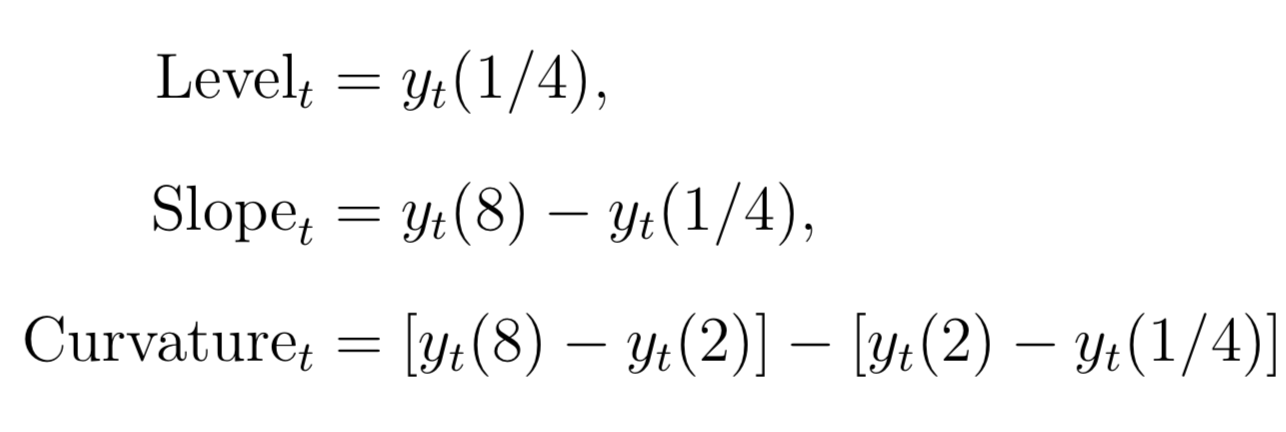
\includegraphics[width=17.86in]{images/level-slope-curvature} \end{center}

The implementation of these is straightforward from the set of spot
rates, so no example is shown here.

\hypertarget{q1}{%
\chapter{Question 1}\label{q1}}

\textbf{Question:}

\emph{What are the time-series properties of the spot rates \(y_t(1)\),
\(y_t(5)\), and \(y_t(10)\)? Report their summary statistics, including
mean, standard deviation, skewness, kurtosis, and the first four
autocorrelation coefficients, and the correlation matrix of the spot
rates. Comment on your results. Also plot them and comment on the time
series patterns.}

In this section, the following packages are used:

\begin{Shaded}
\begin{Highlighting}[]
\KeywordTok{library}\NormalTok{(readr)}
\KeywordTok{library}\NormalTok{(dplyr)}
\KeywordTok{library}\NormalTok{(tidyr)}
\KeywordTok{library}\NormalTok{(ratekit)}
\KeywordTok{library}\NormalTok{(ggplot2)}
\KeywordTok{library}\NormalTok{(broom)}
\KeywordTok{library}\NormalTok{(purrr)}
\end{Highlighting}
\end{Shaded}

We will need the data for the \(y_t(1)\), \(y_t(5)\), and \(y_t(10)\)
spot rates. These have already been calculated in the script referenced
in \ref{spot-rates}, so we can just load them in.

\begin{Shaded}
\begin{Highlighting}[]
\NormalTok{rates_and_prices <-}\StringTok{ }\KeywordTok{read_rds}\NormalTok{(}\StringTok{"data/computed/rates_and_prices.rds"}\NormalTok{)}
\NormalTok{n <-}\StringTok{ }\KeywordTok{c}\NormalTok{(}\StringTok{"1"}\NormalTok{, }\StringTok{"5"}\NormalTok{, }\StringTok{"10"}\NormalTok{)}

\NormalTok{spot_rates_q1 <-}\StringTok{ }\NormalTok{rates_and_prices }\OperatorTok
\StringTok{  }\KeywordTok{filter}\NormalTok{(maturity_nm }\OperatorTok\StringTok{ }\NormalTok{n) }\OperatorTok
\StringTok{  }\KeywordTok{unnest}\NormalTok{() }\OperatorTok
\StringTok{  }\KeywordTok{select}\NormalTok{(}\OperatorTok{-}\NormalTok{zero_price)}

\NormalTok{spot_rates_q1}
\end{Highlighting}
\end{Shaded}

\begin{verbatim}
## # A tibble: 1,377 x 4
##   maturity maturity_nm date       spot_rate
##      <dbl> <chr>       <date>         <dbl>
## 1        1 1           1980-01-31    0.118 
## 2        1 1           1980-02-29    0.145 
## 3        1 1           1980-03-31    0.151 
## 4        1 1           1980-04-30    0.107 
## 5        1 1           1980-05-30    0.0871
## # ... with 1,372 more rows
\end{verbatim}

\hypertarget{summary-statistics}{%
\section{Summary Statistics}\label{summary-statistics}}

Reported below are summary statistics on the three spot rate series.

\begin{tabular}{rrrrr}
\toprule
Maturity & Mean & Standard Deviation & Kurtosis & Skewness\\
\midrule
1 & 0.0480538 & 0.0375029 & 2.913858 & 0.6505396\\
5 & 0.0566592 & 0.0345430 & 2.567191 & 0.5659543\\
10 & 0.0627654 & 0.0314939 & 2.586681 & 0.5793584\\
\bottomrule
\end{tabular}

Unsurprisingly, the average spot rate increases with the maturity, but
interestingly, the shorter maturity spot rates have higher volatility.
The kurtosis of all three are less than that of a normal distribution,
but the 1 year maturity is very close. All three are right-skewed, with
longer right tails, which makes sense considering extremely high
interest rate periods do happen, but are rare.

\hypertarget{autocorrelations}{%
\section{Autocorrelations}\label{autocorrelations}}

The first four autocorrelation correlation coefficients of the 3 series
are reported below, along with a plot of the ACF for the series. Each of
the series are highly autocorrelated.

\begin{tabular}{r|r|r|r|r}
\hline
Maturity & Lag 1 & Lag 2 & Lag 3 & Lag 4\\
\hline
1 & 0.9878979 & 0.9697433 & 0.9527499 & 0.9411647\\
\hline
5 & 0.9911143 & 0.9791933 & 0.9686252 & 0.9599084\\
\hline
10 & 0.9906205 & 0.9793246 & 0.9691974 & 0.9606667\\
\hline
\end{tabular}

By looking at the entire ACF, we can see that the amount of
autocorrelation increases in maturity. At farther out lags, 1 is less
autocorrelated than 5 and 5 less than 10.

\begin{figure}

{\centering 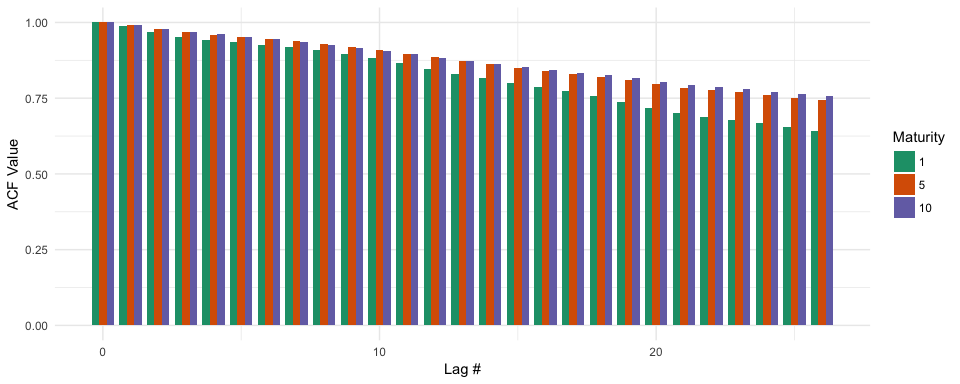
\includegraphics{final-project-book_files/figure-latex/unnamed-chunk-25-1} 

}

\caption{ACF for the 1, 5, and 10 year spot rates}\label{fig:unnamed-chunk-25}
\end{figure}

\hypertarget{correlations}{%
\section{Correlations}\label{correlations}}

Moving on to correlations, it is clear that the the series are
\emph{highly} correlated. This should not be surprising whatsoever.
Intuitively, the 1 year is more correlated with the 5 year than with the
10 year.

\begin{tabular}{l|r|r|r}
\hline
  & 1 & 5 & 10\\
\hline
1 & 1.0000000 & 0.9783620 & 0.9539364\\
\hline
5 & 0.9783620 & 1.0000000 & 0.9932312\\
\hline
10 & 0.9539364 & 0.9932312 & 1.0000000\\
\hline
\end{tabular}

\hypertarget{time-series-visualizations}{%
\section{Time Series Visualizations}\label{time-series-visualizations}}

A look at the time series of the three series confirms the highly
autocorrelated and correlated nature of the three series. 1 year spot
rates are almost always below the longer maturity rates, as one would
expect. Since 2010, 1 year spot rates have been incredibly low, but have
started to pick back up in the last few years.

\begin{figure}

{\centering 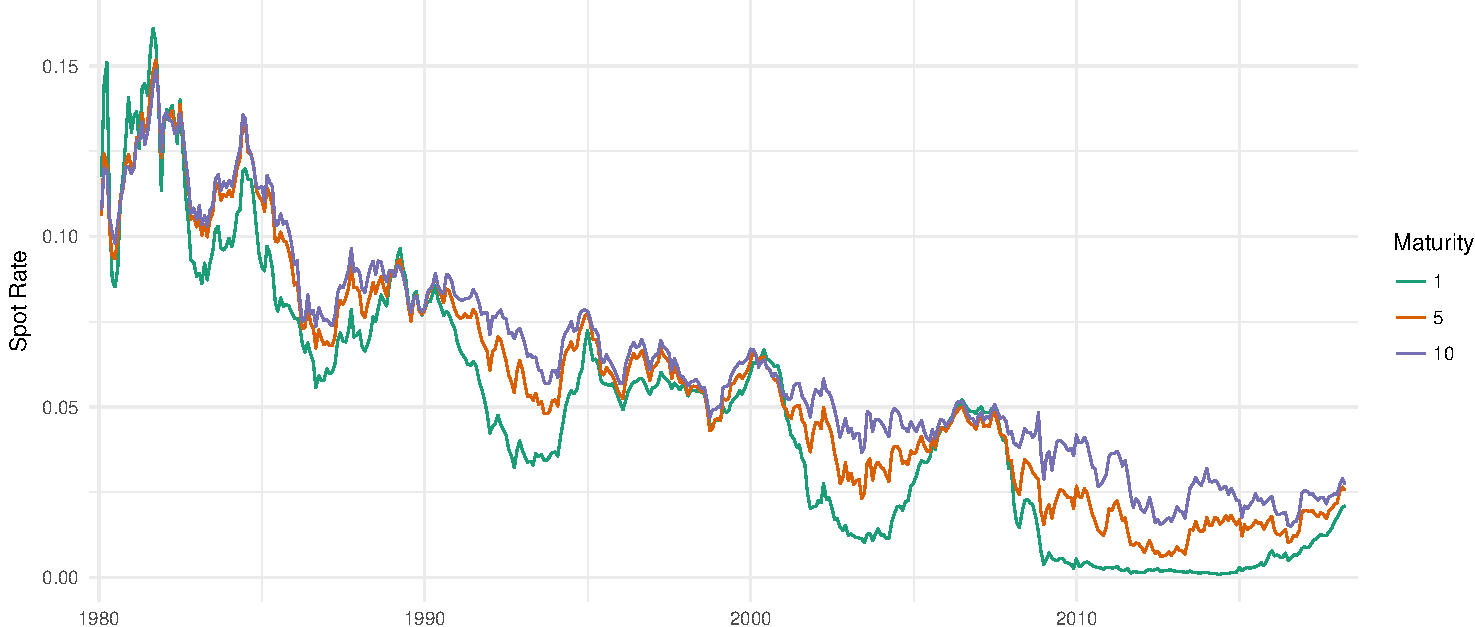
\includegraphics{final-project-book_files/figure-latex/unnamed-chunk-27-1} 

}

\caption{A look at the 1, 5, and 10 year spot rates over time}\label{fig:unnamed-chunk-27}
\end{figure}

\hypertarget{q2}{%
\chapter{Question 2}\label{q2}}

\textbf{Question:}

\emph{Can the three yield curve factors explain the time-series
variation in spot rates? Regress \(y_t(1)\) on a constant and \(X_t\)
and comment on the regression statistics. Perform the same analysis for
\(y_t(5)\) and \(y_t(10)\).}

In this section, the following packages are used:

\begin{Shaded}
\begin{Highlighting}[]
\KeywordTok{library}\NormalTok{(readr)}
\KeywordTok{library}\NormalTok{(dplyr)}
\KeywordTok{library}\NormalTok{(tidyr)}
\KeywordTok{library}\NormalTok{(ratekit)}
\KeywordTok{library}\NormalTok{(ggplot2)}
\KeywordTok{library}\NormalTok{(broom)}
\KeywordTok{library}\NormalTok{(purrr)}
\end{Highlighting}
\end{Shaded}

We will need the data for the \(y_t(1)\), \(y_t(5)\), and \(y_t(10)\)
spot rates along with the yield curve factors. These have already been
calculated in the scripts referenced in \ref{spot-rates} and
\ref{yield-curve-factors} so we can just load them in.

\begin{Shaded}
\begin{Highlighting}[]
\NormalTok{rates_and_prices    <-}\StringTok{ }\KeywordTok{read_rds}\NormalTok{(}\StringTok{"data/computed/rates_and_prices.rds"}\NormalTok{)}
\NormalTok{yield_curve_factors <-}\StringTok{ }\KeywordTok{read_rds}\NormalTok{(}\StringTok{"data/computed/yield_curve_factors.rds"}\NormalTok{)}
\NormalTok{n <-}\StringTok{ }\KeywordTok{c}\NormalTok{(}\StringTok{"1"}\NormalTok{, }\StringTok{"5"}\NormalTok{, }\StringTok{"10"}\NormalTok{)}

\NormalTok{spot_rates_q2 <-}\StringTok{ }\NormalTok{rates_and_prices }\OperatorTok
\StringTok{  }\CommentTok{#filter(maturity_nm %in% n) %>%}
\StringTok{  }\KeywordTok{unnest}\NormalTok{() }\OperatorTok
\StringTok{  }\KeywordTok{select}\NormalTok{(}\OperatorTok{-}\NormalTok{zero_price)}

\NormalTok{spot_rates_q2}
\end{Highlighting}
\end{Shaded}

\begin{verbatim}
## # A tibble: 6,426 x 4
##   maturity maturity_nm date       spot_rate
##      <dbl> <chr>       <date>         <dbl>
## 1   0.0833 1/12        1980-01-31    0.126 
## 2   0.0833 1/12        1980-02-29    0.136 
## 3   0.0833 1/12        1980-03-31    0.161 
## 4   0.0833 1/12        1980-04-30    0.116 
## 5   0.0833 1/12        1980-05-30    0.0795
## # ... with 6,421 more rows
\end{verbatim}

\hypertarget{regression}{%
\section{Regression}\label{regression}}

Using the concept of multiple models from the book,
\href{http://r4ds.had.co.nz/many-models.html}{\texttt{R\ 4\ Data\ Science}},
implementing these regressions in R is incredibly straightforward.
First, we shard the series into separate data frames.

\begin{Shaded}
\begin{Highlighting}[]
\NormalTok{nested_spot <-}\StringTok{ }\NormalTok{spot_rates_q2 }\OperatorTok
\StringTok{  }\CommentTok{# Add on the curve factors}
\StringTok{  }\KeywordTok{left_join}\NormalTok{(yield_curve_factors, }\DataTypeTok{by =} \StringTok{"date"}\NormalTok{) }\OperatorTok
\StringTok{  }
\StringTok{  }\CommentTok{# Group by maturity and nest}
\StringTok{  }\KeywordTok{group_by}\NormalTok{(maturity) }\OperatorTok
\StringTok{  }\KeywordTok{select}\NormalTok{(}\OperatorTok{-}\NormalTok{maturity_nm, }\OperatorTok{-}\NormalTok{date) }\OperatorTok
\StringTok{  }\KeywordTok{nest}\NormalTok{()}
\end{Highlighting}
\end{Shaded}

Then we apply the linear model to each shard. The far right column,
\texttt{model} contains the results of the linear models. I went ahead
and calculated models for every maturity because I am going to use them
in some exploration later.

\begin{Shaded}
\begin{Highlighting}[]
\NormalTok{nested_models <-}\StringTok{ }\NormalTok{nested_spot }\OperatorTok
\StringTok{  }\KeywordTok{mutate}\NormalTok{(}\DataTypeTok{model =} \KeywordTok{map}\NormalTok{(data, }\OperatorTok{~}\StringTok{ }\KeywordTok{lm}\NormalTok{(spot_rate }\OperatorTok{~}\StringTok{ }\NormalTok{level }\OperatorTok{+}\StringTok{ }\NormalTok{slope }\OperatorTok{+}\StringTok{ }\NormalTok{curvature, }\DataTypeTok{data =}\NormalTok{ .x)))}

\NormalTok{nested_models}
\end{Highlighting}
\end{Shaded}

\begin{verbatim}
## # A tibble: 14 x 3
##    maturity data               model   
##       <dbl> <list>             <list>  
##  1   0.0833 <tibble [459 x 4]> <S3: lm>
##  2   0.25   <tibble [459 x 4]> <S3: lm>
##  3   0.917  <tibble [459 x 4]> <S3: lm>
##  4   1      <tibble [459 x 4]> <S3: lm>
##  5   2      <tibble [459 x 4]> <S3: lm>
##  6   2.92   <tibble [459 x 4]> <S3: lm>
##  7   3      <tibble [459 x 4]> <S3: lm>
##  8   4.92   <tibble [459 x 4]> <S3: lm>
##  9   5      <tibble [459 x 4]> <S3: lm>
## 10   6.92   <tibble [459 x 4]> <S3: lm>
## 11   7      <tibble [459 x 4]> <S3: lm>
## 12   8      <tibble [459 x 4]> <S3: lm>
## 13   9.92   <tibble [459 x 4]> <S3: lm>
## 14  10      <tibble [459 x 4]> <S3: lm>
\end{verbatim}

\hypertarget{one-year-spot-rate}{%
\section{One Year Spot Rate}\label{one-year-spot-rate}}

As you can see below, all estimates for the 1 year spot rate model are
highly significant, and the Adjusted \(R^2\) is nearing 100\%,
suggesting that the model can explain essentially all of the variation
in the spot rate.

\begin{tabular}{l|r|r|r|r}
\hline
Term & Estimate & Standard Error & Statistic & P-Value\\
\hline
(Intercept) & 0.001014021 & 0.0001280165 & 7.921022 & 1.8e-14\\
\hline
level & 0.989941953 & 0.0015226534 & 650.142657 & 0.0e+00\\
\hline
slope & 0.264774017 & 0.0034323179 & 77.141460 & 0.0e+00\\
\hline
curvature & -0.428350107 & 0.0057618892 & -74.341954 & 0.0e+00\\
\hline
\end{tabular}

\begin{tabular}{r|r|r}
\hline
R Squared & R Squared Adj & Residual Std Error\\
\hline
0.9995224 & 0.9995193 & 0.0008223\\
\hline
\end{tabular}

A chart of the realized VS predicted time series confirms how well the
variation is explained. It is important to remember that this model is
not predicting future rates, and is simply used to gather intuition
about past rates.

\begin{figure}
\centering
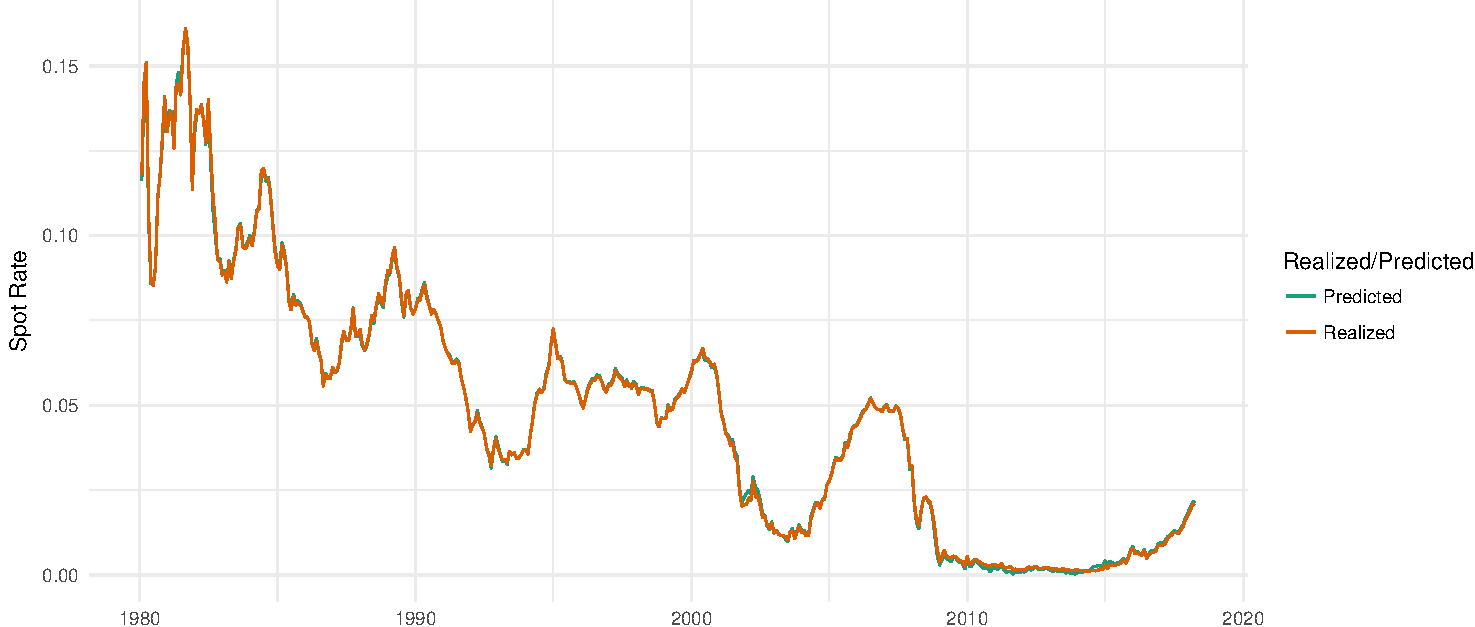
\includegraphics{final-project-book_files/figure-latex/unnamed-chunk-35-1.pdf}
\caption{\label{fig:unnamed-chunk-35}One year spot rate: In sample
predictions VS realized}
\end{figure}

\hypertarget{five-year-spot-rate}{%
\section{Five Year Spot Rate}\label{five-year-spot-rate}}

The model for the 5 year rate is similar to the 1 year rate in terms of
explanatory power.

\begin{tabular}{l|r|r|r|r}
\hline
Term & Estimate & Standard Error & Statistic & P-Value\\
\hline
(Intercept) & -0.001326488 & 0.0001178948 & -11.25146 & 0\\
\hline
level & 1.010756975 & 0.0014022642 & 720.80351 & 0\\
\hline
slope & 0.862622600 & 0.0031609403 & 272.90063 & 0\\
\hline
curvature & -0.237885069 & 0.0053063231 & -44.83049 & 0\\
\hline
\end{tabular}

\begin{tabular}{r|r|r}
\hline
R Squared & R Squared Adj & Residual Std Error\\
\hline
0.9995226 & 0.9995194 & 0.0007572\\
\hline
\end{tabular}

\begin{figure}
\centering
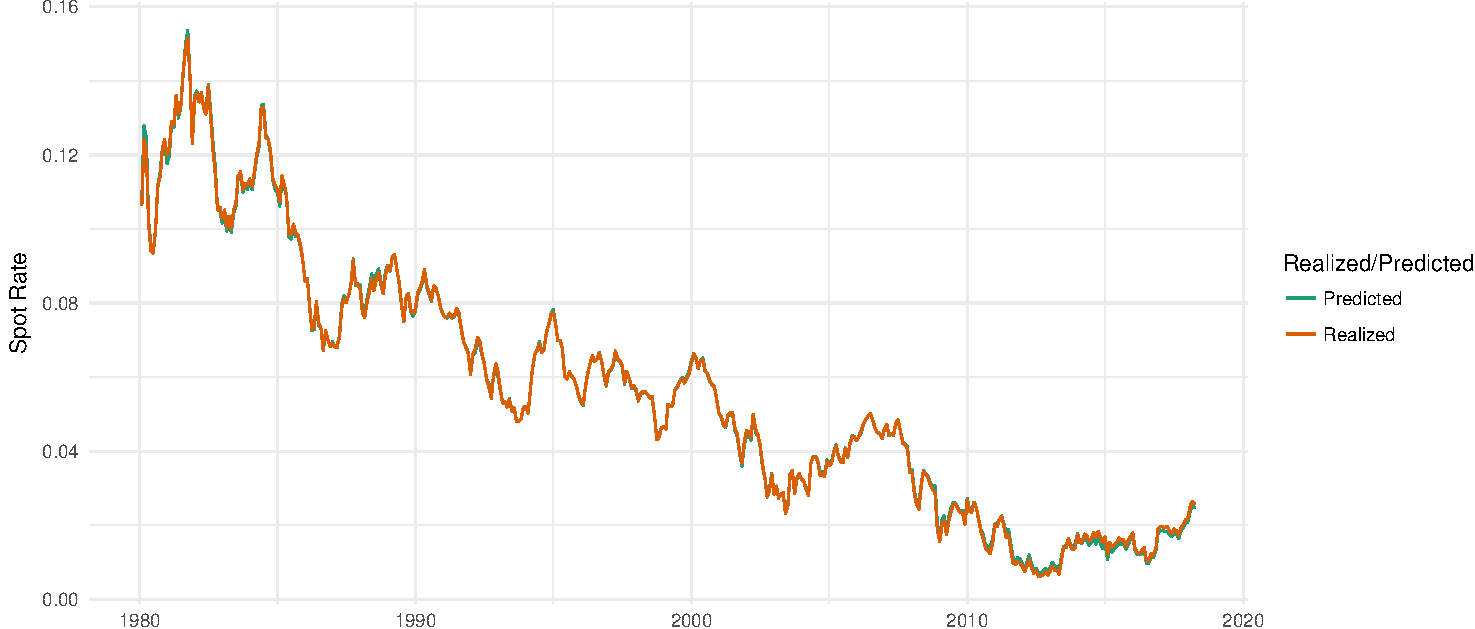
\includegraphics{final-project-book_files/figure-latex/unnamed-chunk-38-1.pdf}
\caption{\label{fig:unnamed-chunk-38}Five year spot rate: In sample
predictions VS realized}
\end{figure}

\hypertarget{ten-year-spot-rate}{%
\section{Ten Year Spot Rate}\label{ten-year-spot-rate}}

And again, the 10 year model performs well too.

\begin{tabular}{l|r|r|r|r}
\hline
Term & Estimate & Standard Error & Statistic & P-Value\\
\hline
(Intercept) & 0.001285415 & 9.632731e-05 & 13.34424 & 0\\
\hline
level & 0.990119282 & 1.145736e-03 & 864.17722 & 0\\
\hline
slope & 1.041806029 & 2.582683e-03 & 403.38126 & 0\\
\hline
curvature & 0.101703126 & 4.335593e-03 & 23.45772 & 0\\
\hline
\end{tabular}

\begin{tabular}{r|r|r}
\hline
R Squared & R Squared Adj & Residual Std Error\\
\hline
0.9996166 & 0.9996141 & 0.0006187\\
\hline
\end{tabular}

\begin{figure}
\centering
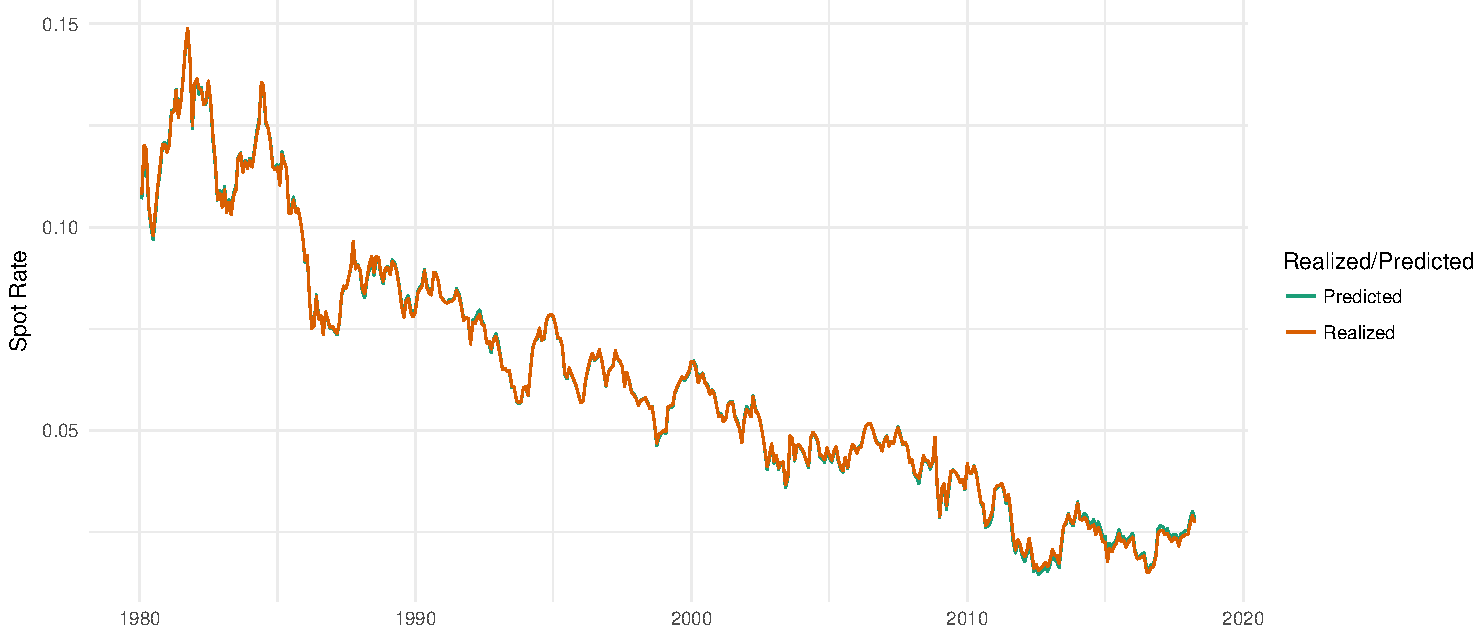
\includegraphics{final-project-book_files/figure-latex/unnamed-chunk-41-1.pdf}
\caption{\label{fig:unnamed-chunk-41}Ten year spot rate: In sample
predictions VS realized}
\end{figure}

\hypertarget{decomposing-the-spot-curve}{%
\section{Decomposing the Spot Curve}\label{decomposing-the-spot-curve}}

Although not specifically asked for, I thought it might be interesting
to decompose and plot the spot curve at a few particular points in time.
We will need a few functions to do so. The functions essentially allow
us to abstract away all the work so that we can just check out the spot
rate graph at any date.

\begin{Shaded}
\begin{Highlighting}[]
\NormalTok{extract_rates <-}\StringTok{ }\ControlFlowTok{function}\NormalTok{(.rates_and_prices, .date) \{}
\NormalTok{  .rates_and_prices }\OperatorTok
\StringTok{    }\KeywordTok{unnest}\NormalTok{() }\OperatorTok
\StringTok{    }\KeywordTok{as_tbl_time}\NormalTok{(date) }\OperatorTok
\StringTok{    }\KeywordTok{group_by}\NormalTok{(maturity) }\OperatorTok
\StringTok{    }\KeywordTok{filter_time}\NormalTok{(}\OperatorTok{~}\NormalTok{.date) }\OperatorTok
\StringTok{    }\KeywordTok{select}\NormalTok{(}\OperatorTok{-}\NormalTok{zero_price)}
\NormalTok{\}}
\end{Highlighting}
\end{Shaded}

\begin{Shaded}
\begin{Highlighting}[]
\NormalTok{tidy_models <-}\StringTok{ }\ControlFlowTok{function}\NormalTok{(.nested_models, .date) \{}
\NormalTok{  coefs <-}\StringTok{ }\NormalTok{.nested_models }\OperatorTok
\StringTok{    }\KeywordTok{mutate}\NormalTok{(}\DataTypeTok{coef =} \KeywordTok{map}\NormalTok{(model, tidy)) }\OperatorTok
\StringTok{    }\KeywordTok{unnest}\NormalTok{(coef) }\OperatorTok
\StringTok{    }\KeywordTok{select}\NormalTok{(maturity, term, estimate) }\OperatorTok
\StringTok{    }\KeywordTok{spread}\NormalTok{(term, estimate) }\OperatorTok
\StringTok{    }\KeywordTok{select}\NormalTok{(}\OperatorTok{-}\StringTok{`}\DataTypeTok{(Intercept)}\StringTok{`}\NormalTok{)}
  
\NormalTok{  yield_fct <-}\StringTok{ }\NormalTok{yield_curve_factors }\OperatorTok
\StringTok{    }\KeywordTok{as_tbl_time}\NormalTok{(date) }\OperatorTok
\StringTok{    }\KeywordTok{filter_time}\NormalTok{(}\OperatorTok{~}\NormalTok{.date)}
  
  \CommentTok{# Multiply the date's yield curve factors by the coefficients to get the}
  \CommentTok{# decomp of the term}
\NormalTok{  decomp <-}\StringTok{ }\NormalTok{coefs }\OperatorTok
\StringTok{    }\KeywordTok{mutate}\NormalTok{(}\DataTypeTok{level =}\NormalTok{ level }\OperatorTok{*}\StringTok{ }\NormalTok{yield_fct}\OperatorTok{$}\NormalTok{level,}
           \DataTypeTok{slope =}\NormalTok{ slope }\OperatorTok{*}\StringTok{ }\NormalTok{yield_fct}\OperatorTok{$}\NormalTok{slope,}
           \DataTypeTok{curvature =}\NormalTok{ curvature }\OperatorTok{*}\StringTok{ }\NormalTok{yield_fct}\OperatorTok{$}\NormalTok{curvature)}
  
\NormalTok{  decomp}
\NormalTok{\}}
\end{Highlighting}
\end{Shaded}

\begin{Shaded}
\begin{Highlighting}[]
\NormalTok{tidy_decomposed_spot_rate <-}\StringTok{ }\ControlFlowTok{function}\NormalTok{(.rates_and_prices, .nested_models, .date) \{}
\NormalTok{  .rates_and_prices }\OperatorTok\StringTok{ }
\StringTok{    }\KeywordTok{extract_rates}\NormalTok{(.date) }\OperatorTok\StringTok{ }
\StringTok{    }\KeywordTok{left_join}\NormalTok{(}\KeywordTok{tidy_models}\NormalTok{(.nested_models, .date), }\StringTok{"maturity"}\NormalTok{) }\OperatorTok
\StringTok{    }\KeywordTok{gather}\NormalTok{(}\StringTok{"line"}\NormalTok{, }\StringTok{"value"}\NormalTok{, }\OperatorTok{-}\NormalTok{(maturity}\OperatorTok{:}\NormalTok{date)) }\OperatorTok
\StringTok{    }\KeywordTok{select}\NormalTok{(maturity, line, value)}
\NormalTok{\}}
\end{Highlighting}
\end{Shaded}

What would these three functions work together to give? Well, for
example, we can try looking at January of 2012. For that date, we get
the spot curve values along with the level, slope and curvature
components from each maturity's model.

\begin{Shaded}
\begin{Highlighting}[]
\NormalTok{rates_and_prices }\OperatorTok
\StringTok{  }\KeywordTok{tidy_decomposed_spot_rate}\NormalTok{(nested_models, }\StringTok{"2012-01"}\NormalTok{) }\OperatorTok
\StringTok{  }\KeywordTok{spread}\NormalTok{(line, value)}
\end{Highlighting}
\end{Shaded}

\begin{verbatim}
## # A tibble: 14 x 5
##    maturity curvature   level     slope spot_rate
##       <dbl>     <dbl>   <dbl>     <dbl>     <dbl>
##  1   0.0833  2.89e- 3 0.00225 -1.04e- 3   0.00254
##  2   0.25    2.51e-18 0.00225  1.25e-18   0.00225
##  3   0.917  -5.37e- 3 0.00222  3.00e- 3   0.00158
##  4   1      -5.65e- 3 0.00222  3.30e- 3   0.00155
##  5   2      -6.59e- 3 0.00225  6.23e- 3   0.00188
##  6   2.92   -5.83e- 3 0.00226  8.12e- 3   0.00307
##  7   3      -5.73e- 3 0.00226  8.26e- 3   0.00320
##  8   4.92   -3.24e- 3 0.00227  1.07e- 2   0.00723
##  9   5      -3.14e- 3 0.00227  1.07e- 2   0.00743
## 10   6.92   -9.69e- 4 0.00226  1.20e- 2   0.0121 
## 11   7      -8.88e- 4 0.00226  1.21e- 2   0.0123 
## 12   8       1.24e-17 0.00225  1.25e- 2   0.0147 
## 13   9.92    1.30e- 3 0.00223  1.30e- 2   0.0188 
## 14  10       1.34e- 3 0.00223  1.30e- 2   0.0190
\end{verbatim}

This extends naturally to charting the decomposed spot rate.

\begin{Shaded}
\begin{Highlighting}[]
\CommentTok{# A charting function with custom themes}
\NormalTok{chart_decomposed_spot_rate <-}\StringTok{ }\ControlFlowTok{function}\NormalTok{(.decomposed_spot) \{}
\NormalTok{  .decomposed_spot }\OperatorTok
\StringTok{    }\KeywordTok{mutate}\NormalTok{(}\DataTypeTok{linetype =} \KeywordTok{case_when}\NormalTok{(}
\NormalTok{      line }\OperatorTok{==}\StringTok{ "spot_rate"} \OperatorTok{~}\StringTok{ "a"}\NormalTok{, }\CommentTok{# this works by alphabetical. first is solid, then dashed}
      \OtherTok{TRUE} \OperatorTok{~}\StringTok{ "b"}
\NormalTok{    )) }\OperatorTok
\StringTok{    }\KeywordTok{ggplot}\NormalTok{(}\KeywordTok{aes}\NormalTok{(}\DataTypeTok{x =}\NormalTok{ maturity, }\DataTypeTok{y =}\NormalTok{ value, }\DataTypeTok{color =}\NormalTok{ line, }\DataTypeTok{linetype =}\NormalTok{ linetype)) }\OperatorTok{+}
\StringTok{    }\KeywordTok{geom_point}\NormalTok{() }\OperatorTok{+}
\StringTok{    }\KeywordTok{geom_smooth}\NormalTok{(}\DataTypeTok{method =} \StringTok{"loess"}\NormalTok{, }\DataTypeTok{se =} \OtherTok{FALSE}\NormalTok{) }\OperatorTok{+}
\StringTok{    }\KeywordTok{theme_minimal}\NormalTok{() }\OperatorTok{+}
\StringTok{    }\KeywordTok{scale_color_brewer}\NormalTok{(}\DataTypeTok{palette =} \StringTok{"Dark2"}\NormalTok{) }\OperatorTok{+}
\StringTok{    }\KeywordTok{labs}\NormalTok{(}\DataTypeTok{x =} \StringTok{"Maturity"}\NormalTok{, }\DataTypeTok{y =} \StringTok{"Component Value"}\NormalTok{, }\DataTypeTok{color =} \StringTok{"Component"}\NormalTok{) }\OperatorTok{+}
\StringTok{    }\KeywordTok{guides}\NormalTok{(}\DataTypeTok{linetype =} \OtherTok{FALSE}\NormalTok{)}
\NormalTok{\}}
\end{Highlighting}
\end{Shaded}

\begin{figure}
\centering
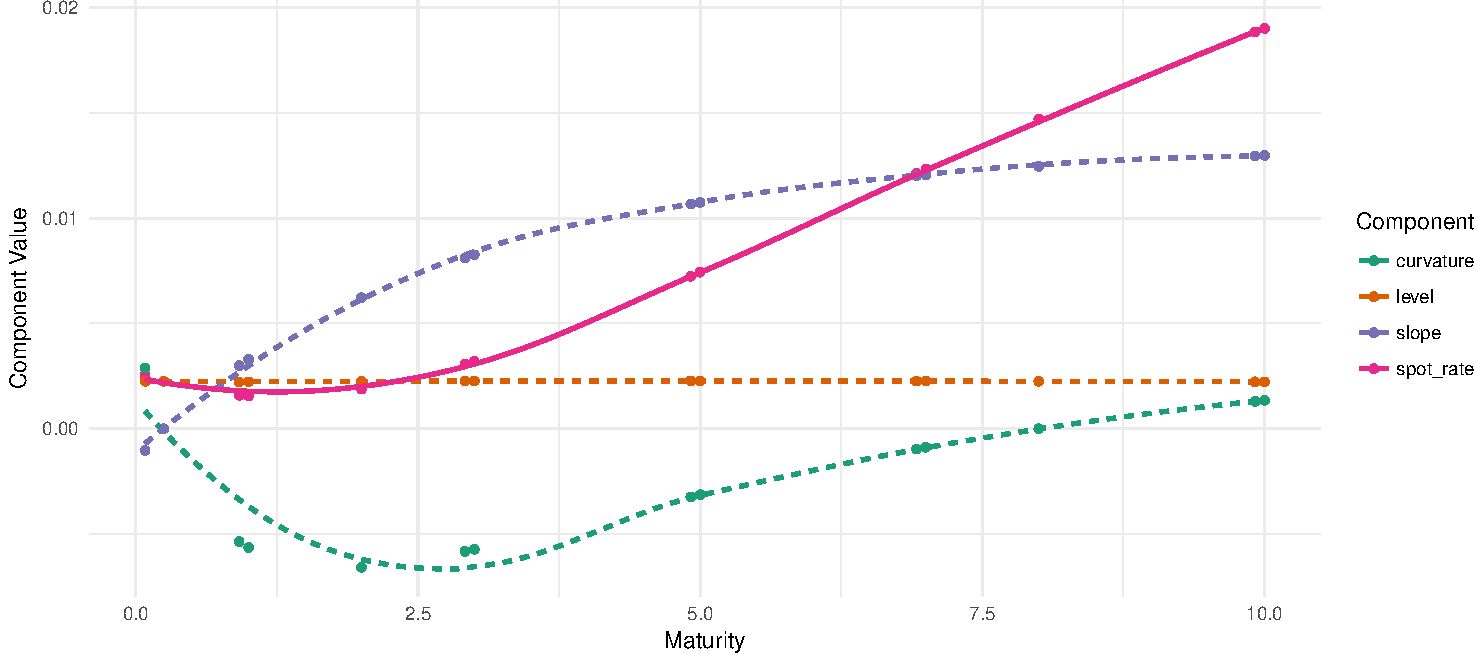
\includegraphics{final-project-book_files/figure-latex/unnamed-chunk-47-1.pdf}
\caption{\label{fig:unnamed-chunk-47}Decomposed Spot Rate for January 2012}
\end{figure}

The spot rate in January of 1981 was definitely an interesting time
period! It's essentially inverted, with lower maturity bonds having
higher spot rates than longer maturity bonds.

\begin{figure}
\centering
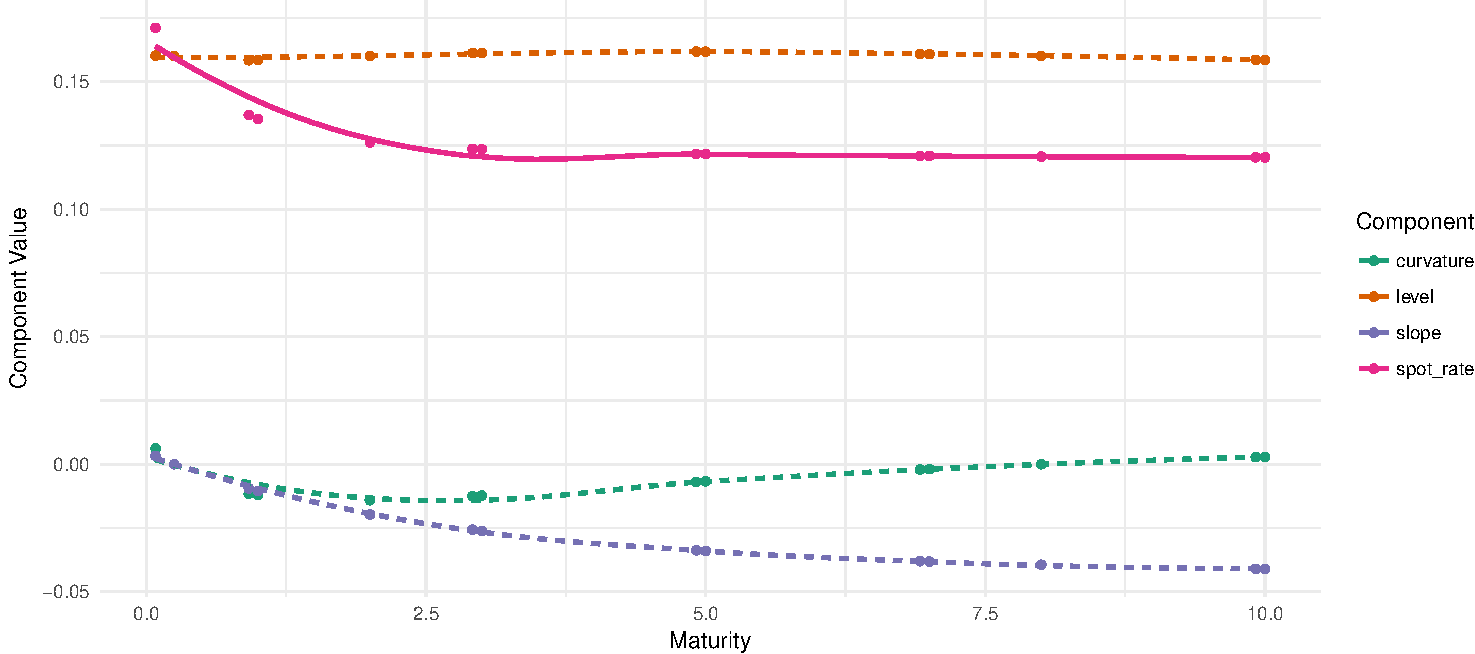
\includegraphics{final-project-book_files/figure-latex/unnamed-chunk-48-1.pdf}
\caption{\label{fig:unnamed-chunk-48}Decomposed Spot Rate for January 1981}
\end{figure}

\hypertarget{coefficient-stability}{%
\section{Coefficient Stability}\label{coefficient-stability}}

Another question worth asking is how stable the coefficients are
throughout time.

\begin{Shaded}
\begin{Highlighting}[]
\KeywordTok{library}\NormalTok{(rsample)}

\NormalTok{splits <-}\StringTok{ }\NormalTok{spot_rates_q2 }\OperatorTok
\StringTok{  }\CommentTok{# Add on the curve factors}
\StringTok{  }\KeywordTok{left_join}\NormalTok{(yield_curve_factors, }\DataTypeTok{by =} \StringTok{"date"}\NormalTok{) }\OperatorTok
\StringTok{  }
\StringTok{  }\CommentTok{# Group by maturity and nest}
\StringTok{  }\KeywordTok{group_by}\NormalTok{(maturity) }\OperatorTok
\StringTok{  }\KeywordTok{select}\NormalTok{(}\OperatorTok{-}\NormalTok{maturity_nm) }\OperatorTok
\StringTok{  }\KeywordTok{nest}\NormalTok{() }\OperatorTok
\StringTok{  }\KeywordTok{filter}\NormalTok{(maturity }\OperatorTok{==}\StringTok{ }\DecValTok{1}\NormalTok{) }\OperatorTok
\StringTok{  }\KeywordTok{unnest}\NormalTok{() }\OperatorTok
\StringTok{  }\KeywordTok{select}\NormalTok{(}\OperatorTok{-}\NormalTok{maturity) }\OperatorTok
\StringTok{  }\KeywordTok{rolling_origin}\NormalTok{(}\DataTypeTok{initial =} \DecValTok{100}\NormalTok{, }\DataTypeTok{assess =} \DecValTok{1}\NormalTok{, }\DataTypeTok{cumulative =} \OtherTok{FALSE}\NormalTok{) }


\NormalTok{splits}\OperatorTok{$}\NormalTok{rolling_models <-}\StringTok{ }\NormalTok{splits}\OperatorTok{$}\NormalTok{splits }\OperatorTok
\StringTok{  }\KeywordTok{map}\NormalTok{(}
    \OperatorTok{~}\StringTok{ }\NormalTok{\{}
      \KeywordTok{lm}\NormalTok{(spot_rate }\OperatorTok{~}\StringTok{ }\NormalTok{level }\OperatorTok{+}\StringTok{ }\NormalTok{slope }\OperatorTok{+}\StringTok{ }\NormalTok{curvature, }\DataTypeTok{data =} \KeywordTok{analysis}\NormalTok{(.x))}
      
\NormalTok{    \}}
\NormalTok{  )}

\NormalTok{splits}\OperatorTok{$}\NormalTok{tidied <-}\StringTok{ }\KeywordTok{map}\NormalTok{(splits}\OperatorTok{$}\NormalTok{rolling_models, tidy)}

\NormalTok{splits}\OperatorTok{$}\NormalTok{enddate <-}\StringTok{ }\KeywordTok{map}\NormalTok{(splits}\OperatorTok{$}\NormalTok{splits, }\OperatorTok{~}\KeywordTok{assessment}\NormalTok{(.x) }\OperatorTok\StringTok{ }\KeywordTok{select}\NormalTok{(date))}
\NormalTok{splits <-}\StringTok{ }\NormalTok{splits }\OperatorTok\StringTok{ }\KeywordTok{unnest}\NormalTok{(enddate)}

\KeywordTok{unnest}\NormalTok{(splits, tidied) }\OperatorTok
\StringTok{  }\KeywordTok{filter}\NormalTok{(term }\OperatorTok{==}\StringTok{ "level"}\NormalTok{) }\OperatorTok
\StringTok{  }\KeywordTok{ggplot}\NormalTok{(}\KeywordTok{aes}\NormalTok{(}\DataTypeTok{x =}\NormalTok{ date, }\DataTypeTok{y =}\NormalTok{ estimate)) }\OperatorTok{+}
\StringTok{  }\KeywordTok{geom_line}\NormalTok{()}
\end{Highlighting}
\end{Shaded}

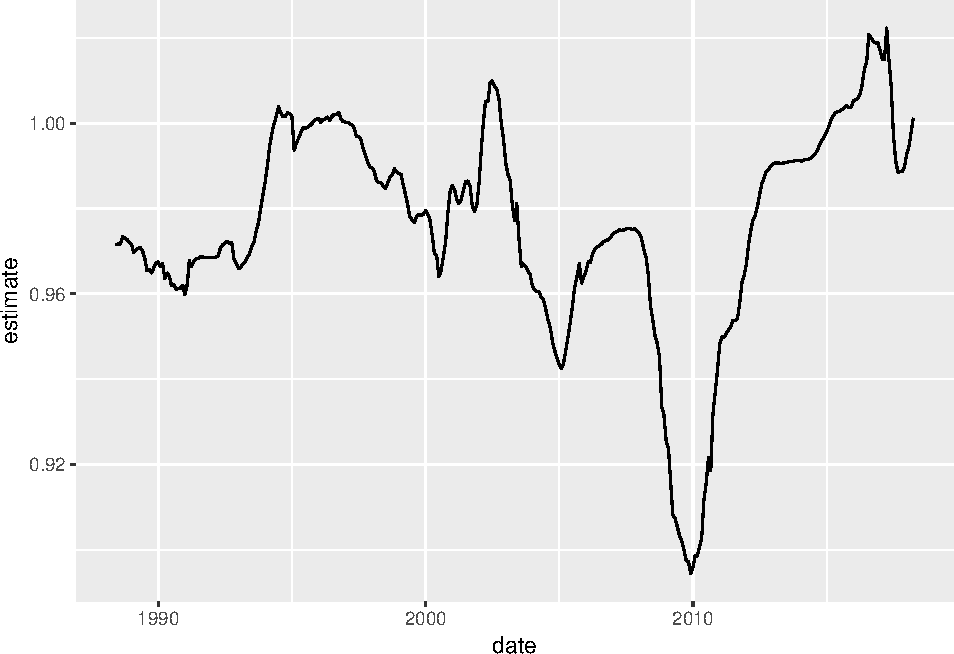
\includegraphics{final-project-book_files/figure-latex/unnamed-chunk-49-1.pdf}

\hypertarget{do-we-need-all-three-factors}{%
\section{Do We Need All Three
Factors?}\label{do-we-need-all-three-factors}}

\bibliography{book.bib,packages.bib}


\end{document}
